\documentclass[conference]{IEEEtran}
% \documentclass{article}
\usepackage{graphicx}
\usepackage{subcaption}
\usepackage{hyperref}
% \renewcommand\thesubsection{}
\usepackage{amsmath}
\begin{document}
\setlength{\parskip}{10pt}

\title{Women's Fashion Recommender System}

\author{
\IEEEauthorblockN{Manish Koppula}
\IEEEauthorblockA{
IMT2020019\\
Manish.koppula@iiitb.ac.in}
\and

\IEEEauthorblockN{Vishnutha Sheela}
\IEEEauthorblockA{
IMT2020057\\
vishnutha.sheela@iiitb.ac.in}
\and

\IEEEauthorblockN{Vivek Tangudu}
\IEEEauthorblockA{
IMT2020110\\
vivek.tangudu@iiitb.ac.in}
\and
\IEEEauthorblockN{Leelavamsikrishna}
\IEEEauthorblockA{
IMT2020111\\
leelavamsikrishna.Sannipalli@iiitb.ac.in}
}

\maketitle

\begin{abstract}
This project aims to revolutionize women's fashion by integrating cutting-edge technologies like LightFM, deep learning-based models, and stable diffusion-based models to enable virtual try-on experiences. Our primary goal is to develop an immersive and personalized fashion recommendation system, empowering users to explore and experiment with diverse clothing styles virtually. Leveraging LightFM's capabilities, we employ collaborative and content-based filtering techniques to tailor recommendations based on users' preferences and interactions. Additionally, deep learning models extract intricate features from fashion items, ensuring accurate matching with user preferences and body types. Furthermore, stable diffusion-based models enable realistic virtual try-on experiences, simulating garment fit and fabric drape with exceptional fidelity. Through seamless integration of these technologies and a user-centric design approach, we aim to redefine the fashion shopping experience, empowering users to effortlessly discover and embrace their unique sense of style.

\end{abstract}
\section{Introduction}

\subsection{Background}

Women's fashion preferences are influenced by a myriad of factors, including personal taste, body type, and occasion. Among these, cultural background plays a significant role in shaping fashion choices. Cultural heritage and traditions inform not only the styles and colors women prefer but also the types of clothing deemed appropriate for various events. With the globalization of fashion and the increasing cultural diversity of customer bases, it becomes essential for fashion recommendation systems to be culturally sensitive and inclusive.

Rent the Runway is an online service that allows women to rent designer dresses and accessories for different occasions. The Rent the Runway ClothFit dataset provides a rich repository of rental transactions, capturing detailed information about user preferences, demographics, and interactions with the platform. This dataset is particularly relevant for developing a recommendation system that can cater to diverse cultural identities, offering personalized suggestions that respect and celebrate these differences.

\subsection{Problem Statement}

The central challenge addressed in this project is the development of a recommendation system that recognizes and respects cultural diversity in fashion preferences. Traditional recommendation algorithms primarily rely on user-item interaction data, which might not sufficiently capture the nuanced influences of cultural background on fashion choices. Given the sparsity of interactions in the Rent the Runway ClothFit dataset—where most users have rented only one or two dresses—it becomes even more challenging to identify patterns that align with cultural sensitivities.

Our goal is to create a recommendation system that goes beyond standard collaborative filtering approaches, integrating cultural context into the personalization process. This involves leveraging the rich attribute data available in the dataset, such as user demographics and detailed garment information, to inform the recommendations. By doing so, we aim to offer tailored fashion suggestions that not only align with individual user preferences but also celebrate and respect their cultural identities and heritage.

\subsection{Objective}

The objective of this project is to develop a recommendation system for women's fashion on Rent the Runway that is culturally sensitive and inclusive. By leveraging the Rent the Runway ClothFit dataset, we aim to create a system that offers personalized fashion recommendations while respecting and celebrating the diverse cultural backgrounds of users. Through the integration of cultural context into the recommendation process, we seek to enhance the user experience and foster a more inclusive fashion environment on the platform.

\section{Dataset Introduction}

In this project, we utilized the Rent the Runway ClothFit dataset, a comprehensive dataset capturing detailed information on clothing rentals and customer interactions. This dataset is particularly well-suited for developing and evaluating a clothing recommendation system due to its real-world relevance and inherent complexity. Rent the Runway is a popular online service that facilitates the rental of designer dresses and accessories, and the dataset provides extensive data on customer preferences, rental history, and garment attributes.

\subsection{Dataset Composition}

The dataset comprises 192,544 rows, representing rental transactions involving 105,571 unique users and 5,850 distinct items. The clothing items span across 68 different categories, providing a diverse range of choices for recommendation algorithms. Key attributes in the dataset include user demographics, garment metadata (such as style, size, and brand), and rental transaction details. Specifically, the attributes include \textit{user\_id}, \textit{bust size}, \textit{item\_id}, \textit{weight}, \textit{rating}, \textit{rented for}, \textit{review\_text}, \textit{body type}, \textit{review\_summary}, \textit{category}, \textit{height}, \textit{size}, \textit{age}, and \textit{review\_date}. This diversity of attributes offers a rich foundation for experimenting with multiple recommendation algorithms, aiming to personalize the rental experience based on individual user profiles and historical interactions.

\subsection{Challenges in the Dataset}

One of the primary challenges presented by the Rent the Runway ClothFit dataset is the sparsity of user-item interactions. A significant proportion of users have rented only one or two dresses, with a median rental count of one per user. This results in a highly sparse user-item interaction matrix, making it difficult for traditional recommendation algorithms to find sufficient patterns and correlations. Additionally, the median item buy count is 14, indicating that while some items are rented frequently, many others have much fewer interactions, further contributing to the sparsity issue. This sparsity poses substantial challenges for collaborative filtering algorithms, which typically depend on a substantial volume of interaction data to generate accurate recommendations. The limited interaction data means that traditional algorithms might struggle to identify patterns and make reliable predictions.

\subsection{Relevance and Practicality}

Despite these challenges, we selected the Rent the Runway ClothFit dataset for several compelling reasons. Firstly, the dataset closely mirrors the conditions that a startup or rapidly growing company might encounter---having limited interactions per user while still needing to provide effective recommendations. This makes our project highly relevant for practical applications in the early stages of business development. Secondly, the dataset's real-world nature ensures that our findings and improvements have direct applicability to similar recommendation systems in the industry.

\subsection{Data Preprocessing}

To effectively utilize the dataset, certain preprocessing steps were necessary. Attributes such as height, weight, and bust size were converted to a consistent format to ensure uniformity in the data. This preprocessing step was crucial for the accurate application of recommendation algorithms, particularly those that utilize user physical characteristics for personalized recommendations.

\subsection{Insights and Opportunities}

The Rent the Runway ClothFit dataset serves as a rich resource for developing and testing cloth recommendation systems. Despite the inherent challenges of data sparsity and the diversity of interactions, it provides a realistic scenario akin to the data landscape faced by emerging companies in the online fashion rental industry. Through careful preprocessing and the application of various recommendation algorithms, this dataset offers valuable insights and opportunities for innovation in personalized fashion recommendations.

\section{Comprehensive Analysis of Recommendation Algorithms}

Our pursuit of enhancing the user experience on Rent the Runway has led us to a thorough exploration and evaluation of a diverse array of recommendation algorithms. Each algorithmic approach has been meticulously designed and implemented to uncover patterns, understand user preferences, and refine the recommendation system. In this comprehensive analysis, we delve into the intricacies of each algorithm, shedding light on its methodology, performance metrics, and insights gleaned from the experimentation process.

\subsection{Content-Based Recommendation System}

At the core of our recommendation system lies the content-based approach, which harnesses the rich textual data embedded within user reviews. Through the application of TF-IDF (Term Frequency-Inverse Document Frequency), we transform textual reviews into numerical embeddings, encapsulating the essence of users' feedback. These embeddings are then subjected to K-means clustering, facilitating the categorization of users based on the similarity of their expressed preferences. When a user seeks a recommendation, the system dynamically identifies the cluster whose preferences resonate with the user's request and suggests dresses that have garnered favor within that cluster. The Silhouette Score, standing at 0.0071, underscores the model's reasonable performance in aligning recommendations with user preferences.

\subsection{Collaborative Filtering}

Collaborative filtering serves as a cornerstone in our recommendation system, aiming to uncover underlying patterns through the analysis of user-item interactions.

\subsubsection{K Nearest Neighbours (KNN)}

K Nearest Neighbours (KNN) stands as a robust approach within collaborative filtering, leveraging a plethora of user features, including age, body measurements, and other relevant attributes. This methodology computes recommendations based on user similarity, discerned through the calculation of Euclidean distance in a multi-dimensional feature space. By identifying users who share similarities with the target user, the algorithm effectively draws on the preferences of these 'neighbours' to generate personalized recommendations. The Mean Reciprocal Rank (MRR) of 0.0052 underscores the algorithm's adeptness at identifying users with similar tastes and recommending items accordingly. Through its comprehensive consideration of user attributes and nuanced understanding of user similarity, KNN emerges as a powerful tool in facilitating tailored recommendations on Rent the Runway.

\subsubsection{Cosine Similarity}

The Cosine Similarity methodology represents another notable approach in collaborative filtering, offering unique insights into product relationships based on user perceptions reflected in reviews. This method involves preprocessing product reviews and harnessing Word2vec for word embeddings, enabling the measurement of how closely products are related in terms of user perception. The resulting Average Precision at 5 of approximately 0.00017 highlights the algorithm's nuanced ability to discern product similarities and make refined recommendations. By capturing subtle nuances in user preferences and product relationships, Cosine Similarity enriches the recommendation process, contributing to an enhanced user experience on Rent the Runway.

\subsubsection{K Means Clustering}

In a similar vein to the content-based approach, K Means Clustering emerges as a compelling strategy within collaborative filtering, facilitating personalized recommendations tailored to distinct user groups. This methodology categorizes users into clusters based on their attributes, fostering a deeper understanding of user preferences and facilitating the delivery of tailored recommendations congruent with each cluster's characteristics. The Silhouette Score of 0.0071 reaffirms the model's capacity for delivering tailored recommendations. By segmenting users into cohesive groups and aligning recommendations with their shared preferences, K Means Clustering offers a nuanced approach to collaborative filtering, enriching the recommendation process and elevating the user experience on Rent the Runway.

\subsubsection{Singular Value Decomposition (SVD)}

Singular Value Decomposition (SVD) stands as a foundational technique within collaborative filtering, offering insights into latent factors that influence user preferences and item appeal. By decomposing the user-item rating matrix, SVD unveils underlying patterns and relationships, facilitating the generation of accurate recommendations. The algorithm's RMSE of 1.41432 reflects a competent grasp of item correlations, crucial for predicting user preferences accurately. Through its adept handling of complex data structures and nuanced understanding of user-item interactions, SVD contributes to the refinement of the recommendation system, fostering a more personalized and engaging user experience on Rent the Runway.

\subsubsection{Multi-Arm Bandit}
Multi-armed bandits are essential for any recommender system to maximise user engagement and utility. It's our tool to understand complex user behaviour. In our model, We have 68 categories of garments in our dataset which are considered arms, The business pulls the arms and the user gives the reward in the form of a rating or just buying the product. 

\textbf{UCB Recommender:}
This algorithm selects arms based on the ucb values given by the formula 
\begin{equation}
    UCB[arm] = \mu[arm] + \sqrt{\frac{\alpha\ln(T[user])}{N[arm]}}
\end{equation}
where $\mu$ is the average rating of the total items present in that arm, and T is the current time step of the user. N is the number of times the business has pulled that category/arm. $\alpha$ is the exploration control factor. We choose $\alpha$ as 1 for the working of the model.

The UCB Recommender selects the top two arms with the highest ucb values and then recommends the users half items from each of the arms.
The items are selected based on their average rating.\\ \\
\textbf{Thompson Sampling:}
This is a probabilistic approach to the multi-armed bandit problem, This will make decisions by sampling from the posterior distribution of the arm's rewards. Each arm is associated with a prior distribution representing beliefs about its reward distribution. After observing outcomes, the prior distributions are updated using Bayes' theorem to obtain posterior distributions. We are using user-buy to update the distributions. For illustration and convergence purposes we have only used 4 categories in the implementation of the model, i.e., Gown, dress, top, and sheath. 
\subsubsection{Deep Learning based Recommendation System}
The deep learning model utilizes user and product embeddings to forecast ratings for user-item interactions. User embeddings are constructed from textual data, such as tokenized text, coupled with numerical features such as height, weight, age, and bust size. Similarly, product embeddings are derived from textual information and numerical attributes like height, weight, age, and rating. These embeddings effectively encapsulate semantic details and user-item interactions, serving as the foundation for the recommendation model.

The neural network architecture comprises three dense layers employing ReLU activation functions. This model is trained using the Adam optimizer and the Mean Squared Error (MSE) loss function. Throughout the training process, the model achieved an MSE of 1.71 on the training dataset and a marginally lower validation loss of 1.63. These results indicate reasonable performance in the prediction of ratings.To predict ratings for a new user, we constructed a new user profile based on their preferences, leveraging the same process used during training to create user embeddings. 
\section{Multi-modal Recommendation System}

\subsection{Data Preparation}

Our study began with meticulous data collection, assembling a diverse dataset comprising user profiles, product specifications, ratings, and associated reviews. The focal point was to create a multi-modal dataset seamlessly integrating textual and visual information. With careful selection, we curated a corpus of 100 images sourced from the esteemed 'Rent the Runway' website, each meticulously paired with corresponding textual reviews to ensure coherence and relevance. This dataset formed the bedrock for our proof-of-concept validation, enabling exploration of the synergies between visual and textual cues in the recommendation process.

\subsection{Model Architecture and Training}

Subsequently, we developed a sophisticated neural network architecture comprising four layers, strategically engineered to harness the multi-modal nature of our dataset. This architecture was meticulously crafted to accommodate inputs from both visual and textual modalities, facilitating seamless integration of information. Through rigorous training over 50 epochs, our model underwent iterative refinement, leveraging advanced optimization techniques to adeptly translate visual inputs into coherent textual representations. Notably, the penultimate layer was tactically designed to encapsulate the semantic essence present in both visual imagery and textual content. This fusion of modalities empowered our model to extract rich semantic representations, enhancing its ability to discern nuanced relationships between images and text.

\subsection{Recommendation Algorithm: LightFM Model}

Utilizing the semantically enriched representation derived from our multi-modal model, we deployed a LightFM model to extract salient features and generate clothing recommendations. The LightFM model, renowned for its versatility in incorporating both user-item interactions and auxiliary data, was well-suited for our multi-modal recommendation framework. To optimize performance, we strategically applied Bayesian Personalized Ranking (BPR) and Weighted Approximate-Rank Pairwise (WARP) loss functions, fine-tuning model parameters to maximize recommendation accuracy. Our efforts yielded a notable precision rate of 0.89 at k = 5, affirming the efficacy of our approach in generating personalized clothing recommendations tailored to individual user preferences.

Our research objectives center on elucidating the effectiveness of our proposed methodology in facilitating personalized dress recommendations that resonate with users on a profound level. We underscore the potential of leveraging larger image datasets and user-generated content to further refine recommendation accuracy and enhance user satisfaction.

Moving forward, we aim to delve into user engagement dynamics, soliciting user-contributed images to enrich our recommendation ecosystem. By deploying innovative models like the CP-ViTon Stable Diffusion, users will be empowered to engage in virtual clothing trials, fostering personalized recommendation experiences aligned with their unique stylistic inclinations and preferences. This iterative refinement underscores our commitment to continuously enhancing the multi-modal recommendation system, ensuring it evolves to meet the dynamic needs and preferences of Rent the Runway users.
\subsection{Results}
We tested our model to give recommendations to a user based on their image and took the top 5 recommendations.
\subsubsection{Existing User}
This is for an existing user, \textit{i.e.}, someone who has already rented at least one item from the store.  
\begin{figure}[!htbp]
  \centering
  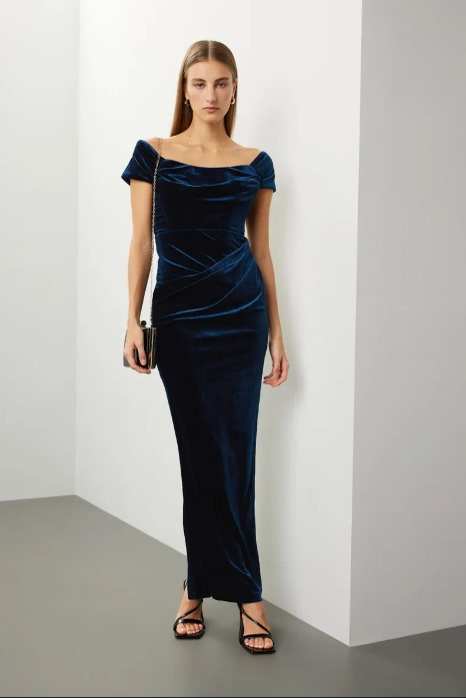
\includegraphics[width=0.4325\textwidth]{t1.jpg}
  \caption{Existing User's Image}
  \label{fig:User}
\end{figure}

\begin{figure}[!htbp]
  \centering
  \begin{subfigure}[b]{0.4\textwidth}
    \centering
    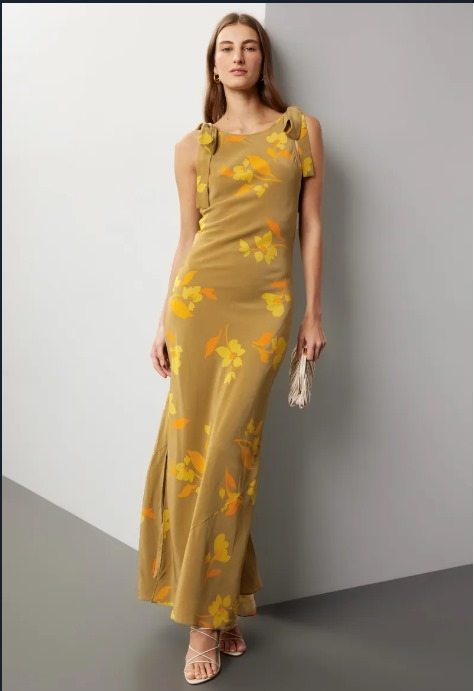
\includegraphics[width=\textwidth]{r1.jpg}
    \caption{Recommendation 1 for existing user }
    \label{fig:Recommendations1}
  \end{subfigure}
  \hfill
  \begin{subfigure}[b]{0.4\textwidth}
    \centering
    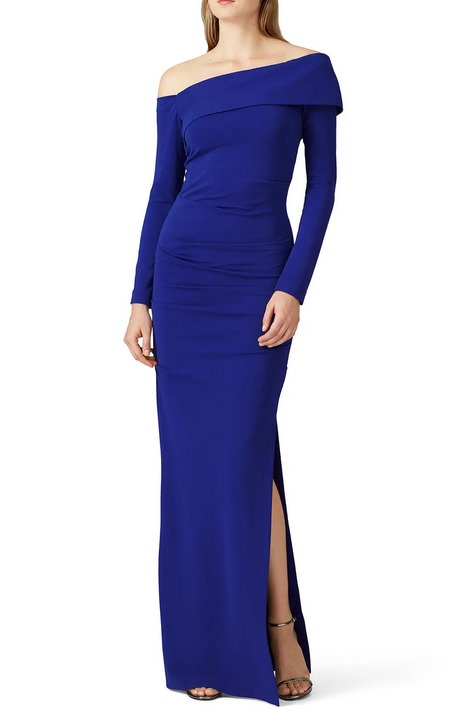
\includegraphics[width=\textwidth]{r2.jpg}
    \caption{Recommendation 2 for existing user}
    \label{fig:Recommendations2}
  \end{subfigure}

\end{figure}

% Somewhere in your document before the figure environment

\begin{figure}[!htbp]
  \centering
  \begin{subfigure}[b]{0.3\textwidth}
    \centering
    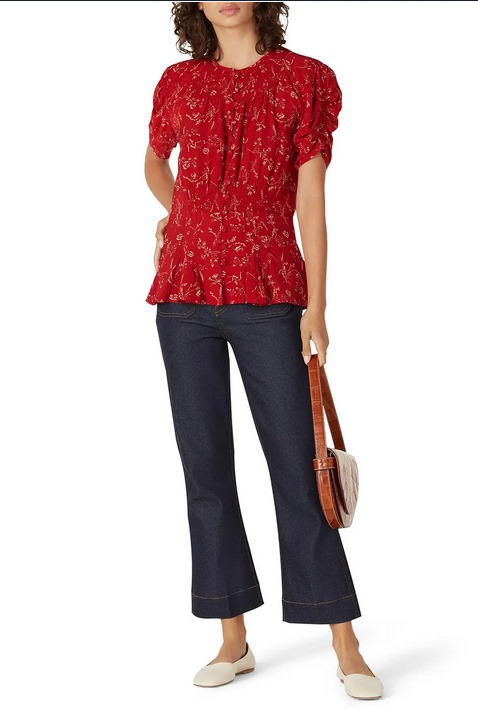
\includegraphics[width=\textwidth]{r3.jpg}
    \caption{Recommendation 3 for existing user}
    \label{fig:Recommendations3}
  \end{subfigure}  
  
  \begin{subfigure}[b]{0.3\textwidth}
    \centering
    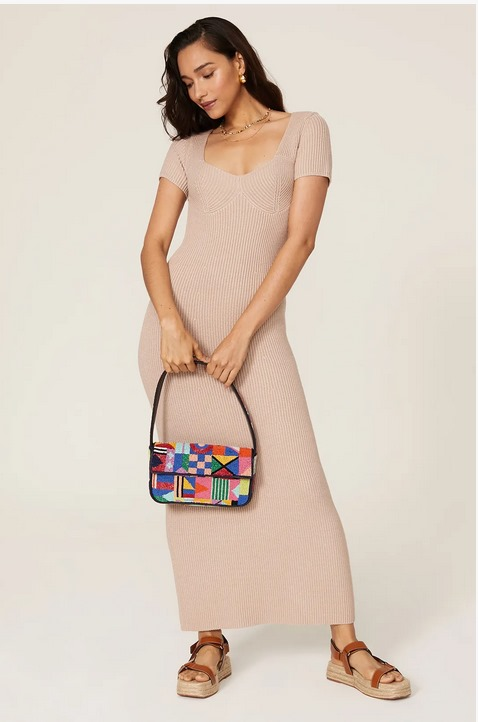
\includegraphics[width=\textwidth]{r4.jpg}
    \caption{Recommendation 4 for existing user}
    \label{fig:Recommendations4}
  \end{subfigure}
  \hfill
  \begin{subfigure}[b]{0.3\textwidth}
    \centering
    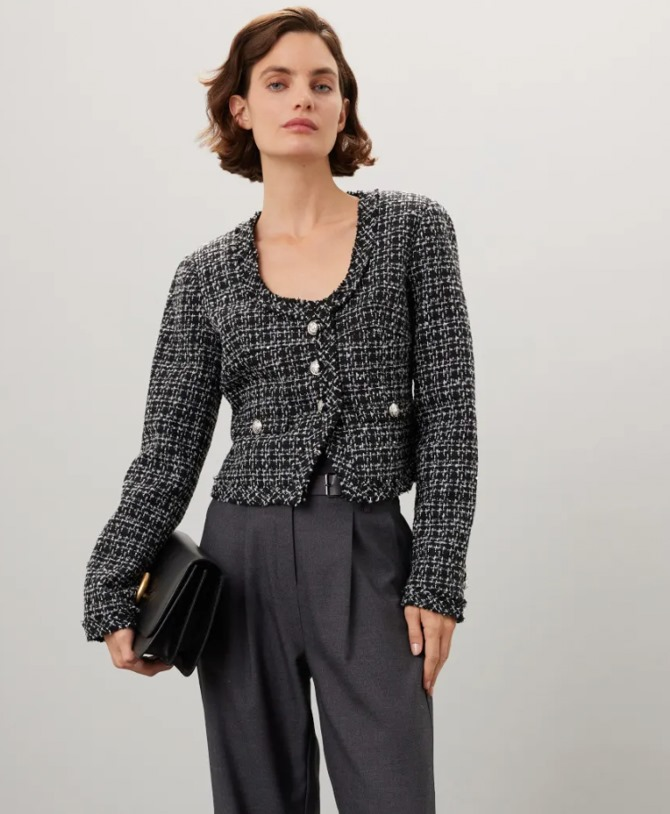
\includegraphics[width=\textwidth]{r5.jpg}
    \caption{Recommendation 5 for existing user}
    \label{fig:Recommendations5}
  \end{subfigure}
  \caption{Top 5 Recommendations for Existing User}
  \label{fig:AllRecommendations}
\end{figure}
\newpage
\subsubsection{New User}
This is for a new user, here, we use k-means clustering algorithm on the latent embeddings we get from the penultimate layer form the neural network that we trained on the image and text embeddings and give the recommendations to the user, along with the try-on.

\begin{figure}[!htbp]
  \centering
  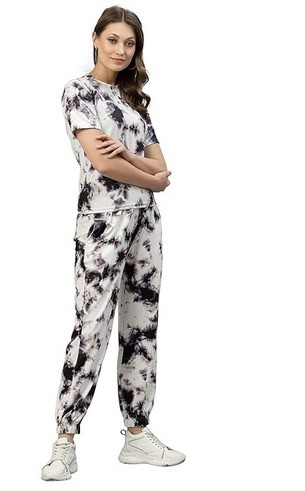
\includegraphics[width=0.375\textwidth]{new1.jpg}
  \caption{New User's Image}
  \label{fig:New User}
\end{figure}

\begin{figure}[!htbp]
  \centering
  \begin{subfigure}[b]{0.5\textwidth}
    \centering
    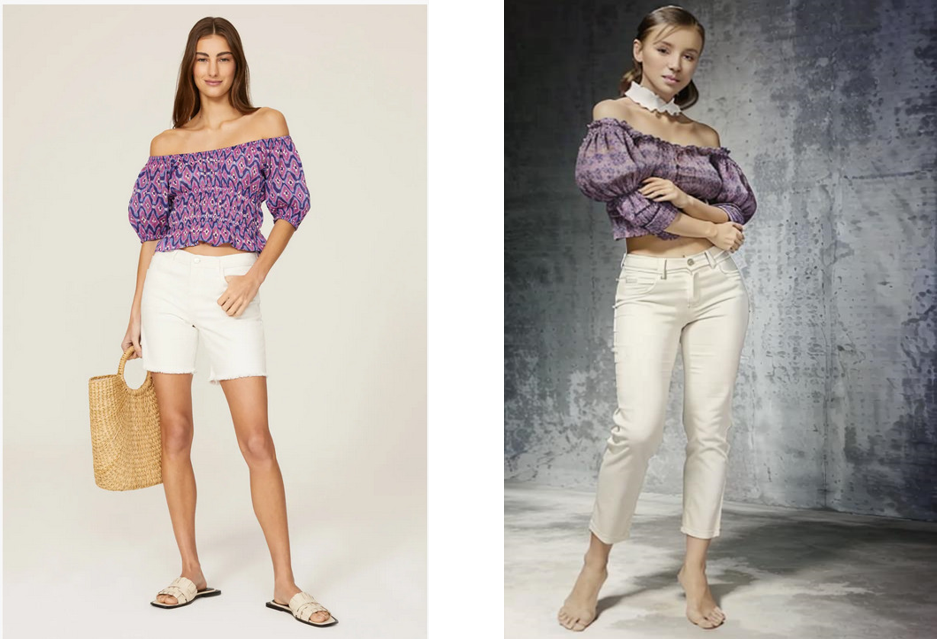
\includegraphics[width=\textwidth]{Picture1.png}
    \caption{Recommendation 1 for new user }
    \label{fig:Recommendations1}
  \end{subfigure}
  \hfill
  \begin{subfigure}[b]{0.5\textwidth}
    \centering
    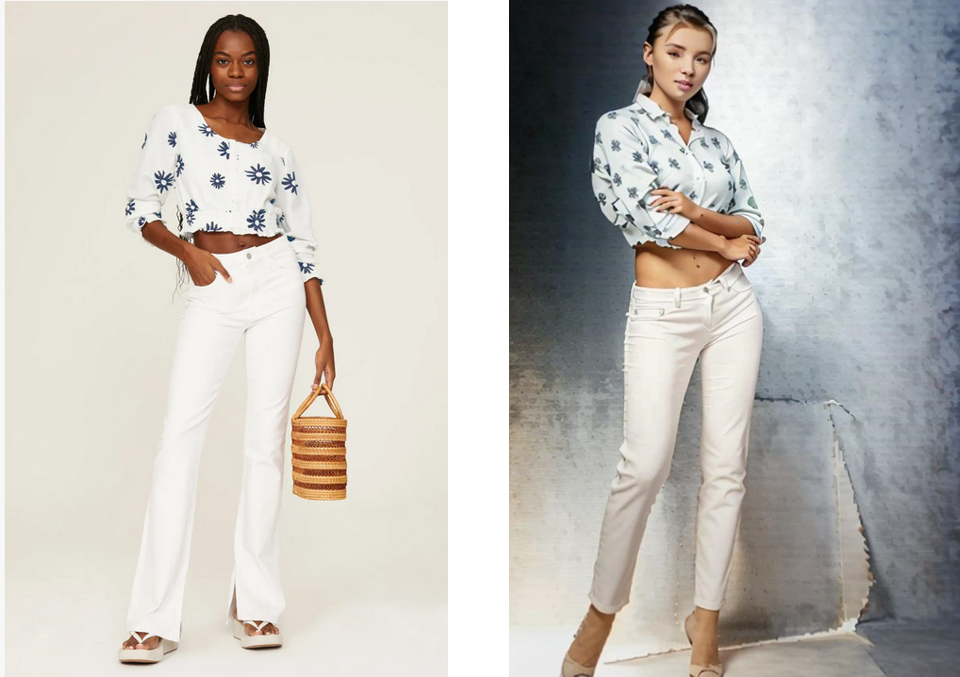
\includegraphics[width=\textwidth]{Picture2.png}
    \caption{Recommendation 2 for new user}
    \label{fig:Recommendations2}
  \end{subfigure}
  \hfill
  \begin{subfigure}[b]{0.5\textwidth}
    \centering
    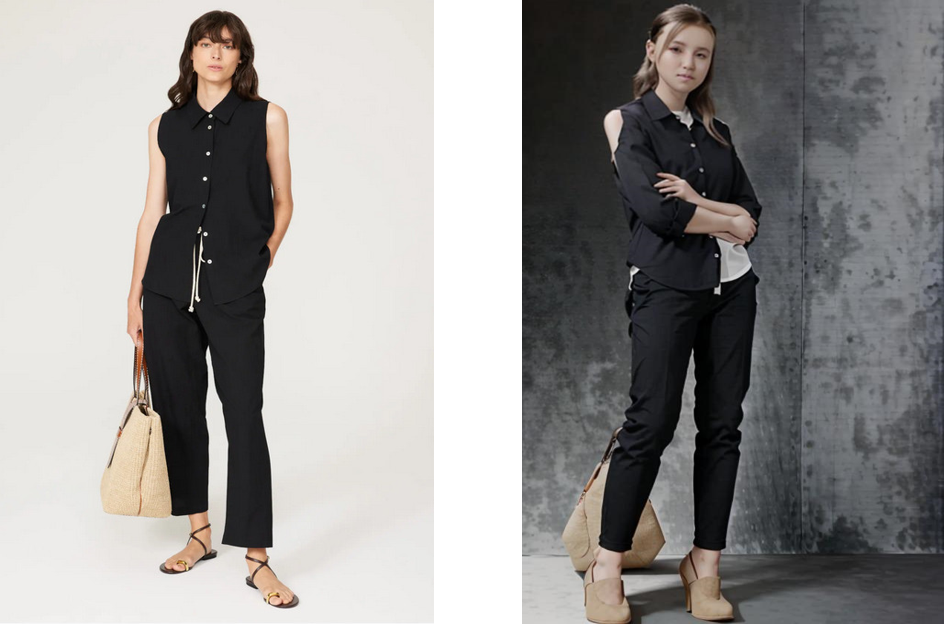
\includegraphics[width=\textwidth]{Picture3.png}
    \caption{Recommendation 3 for new user}
    \label{fig:Recommendations3}
  \end{subfigure}  
  \caption{Top 3 Recommendations and Try-ons}
  \label{fig:AllRecommendations}
\end{figure}


\section{Future Scope and Limitations}
\subsection{Limitations}
\textbf{Gender Bias in Data Representation:} As the system's goal is to recommend clothes specifically for women, there's a chance that the dataset's gender biases will be strengthened. It is imperative to tackle this constraint by proactively pursuing a range of viewpoints and guaranteeing fair representation in the dataset and recommendation algorithms.

\textbf{Restricted Coverage of Fashion Preferences:} Although the recommendation system might be excellent at making dress recommendations based on user reviews and image analysis, its application might be restricted to particular trends or fashion styles that are common in the dataset. This can cause users' specific or evolving fashion tastes to be overlooked.

\textbf{Single-Modal Recommendations:} The system mostly uses image-text fusion for suggestion generation, although attempts have been made to integrate user-generated content and feedback. To improve suggestion diversity and relevance, future iterations can investigate adding more modalities like user preferences, occasion-specific requirements, or social influence.

\textbf{User Adoption and Engagement Challenges:} Encouraging users to actively participate in the recommendation system by submitting photographs and leaving comments may provide adoption issues, especially for users who value their privacy or are reluctant to divulge personal information. Strong user engagement tactics and open communication about data usage and privacy protections are necessary to remove these obstacles.

\subsection{Future Scope}
% \textbf{Personalized Customization:} Expanding beyond dress recommendations, the system could evolve to offer personalized customization options tailored to individual users' body types, style preferences, and occasion-specific requirements. This could include suggesting matching accessories, footwear, or complementary clothing items, enhancing the overall shopping experience.

\textbf{Integrating Social and Cultural Context:}Future versions of the recommendation system may include socio-cultural context analysis to provide recommendations that are inclusive and sensitive to cultural differences, given the growing impact of social and cultural aspects on fashion choices. To improve suggestion relevancy and variety, this may entail utilizing user-generated content, social media trends, and cultural insights.

\textbf{Multi-Modal Fusion for Improved Recommendations:} Adopting a multi-modal strategy and combining various data sources, such as trend research, influencer endorsements, and user reviews, could improve the diversity and accuracy of recommendations even more. Through the use of advanced fusion techniques, such as text-image-audio data, the system is able to offer more comprehensive and customized fashion recommendations based on the interests of each user.


\textbf{Continuous Learning and Adaptation:} In order to make sure the recommendation system stays relevant and sensitive to changing user preferences and fashion trends, it is imperative to implement mechanisms for continual learning and adaptation. This involves employing real-time data analytics, user feedback loops, and machine learning approaches to iteratively improve recommendation algorithms and increase customer happiness. 

\end{document}
